La figura muestra un sólido del primer octante limitado por el cilindro parabólico $x=1-y^2$ y el plano $z=1-y$. Escriba $\iiint_E f\,dV$ en los órdenes $dx\,dz\,dy$ y $dz\,dy\,dx$.

\begingroup
\shorthandoff{>}
\begin{center}
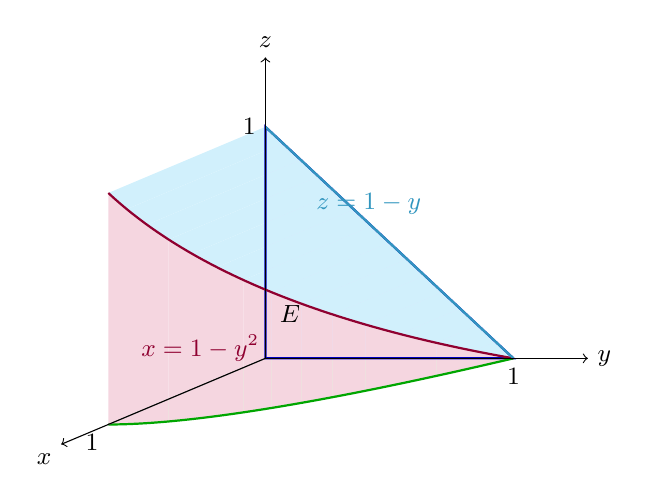
\begin{tikzpicture}[
    x={(-1.9cm,-.8cm)},y={(3cm,0cm)},z={(0cm,2.8cm)},
    scale=1.05,every node/.style={font=\small}]
    \fill[blue!10] (0,0,0) -- (0,1,0) -- (0,0,1) -- cycle;
    \fill[green!13] (0,0,0) -- (1,0,0) --
        plot[domain=0:1,samples=40] ({1-\x*\x},{\x},0) -- cycle;
    \foreach \i in {0,...,13} {
        \pgfmathsetmacro{\ya}{\i/14}
        \pgfmathsetmacro{\yb}{(\i+1)/14}
        \fill[cyan!18]
            (0,\ya,{1-\ya}) -- ({1-\ya*\ya},\ya,{1-\ya}) --
            ({1-\yb*\yb},\yb,{1-\yb}) -- (0,\yb,{1-\yb}) -- cycle;
        \fill[purple!16]
            ({1-\ya*\ya},\ya,0) -- ({1-\yb*\yb},\yb,0) --
            ({1-\yb*\yb},\yb,{1-\yb}) --
            ({1-\ya*\ya},\ya,{1-\ya}) -- cycle;
    }
    \draw[blue!75!black,thick] (0,0,0) -- (0,1,0) -- (0,0,1) -- cycle;
    \draw[green!65!black,thick]
        plot[domain=0:1,samples=45] ({1-\x*\x},{\x},0);
    \draw[purple!75!black,thick]
        plot[domain=0:1,samples=45] ({1-\x*\x},{\x},{1-\x});
    \draw[cyan!75!black,thick] (0,0,1) -- (0,1,0);
    \draw[gray!65] (0,0,0) -- (1,0,0);
    \draw[->] (0,0,0) -- (1.3,0,0) node[below left] {$x$};
    \draw[->] (0,0,0) -- (0,1.3,0) node[right] {$y$};
    \draw[->] (0,0,0) -- (0,0,1.3) node[above] {$z$};
    \node[below left] at (1,0,0) {$1$};
    \node[below] at (0,1,0) {$1$};
    \node[left] at (0,0,1) {$1$};
    \node[purple!75!black,left] at (.72,.47,.25) {$x=1-y^2$};
    \node[cyan!75!black,right] at (.18,.28,.72) {$z=1-y$};
    \node at (.38,.34,.3) {$E$};
\end{tikzpicture}
\end{center}
\endgroup
